
\documentclass[leqno]{article}
\usepackage[top=10em]{geometry}
\usepackage{amsmath}
\usepackage{tikz}
\usepackage{tikz-qtree,tikz-qtree-compat}
\usepackage{graphicx}
\usepackage[margin=1cm]{caption}
\usepackage{paralist}
\usepackage{wrapfig}
\usepackage[colorlinks, linkcolor=purple]{hyperref}
\usepackage{cleveref}

\title{Compressive Saliency Sensing: sampling near the edges}
\date{}
\author{Scott Sievert\\ \texttt{sieve121@umn.edu}}

\begin{document}


    \maketitle
    {\hypersetup{linkcolor=blue} \tableofcontents}
    \hrulefill

    \section{One Dimension}
        In one dimension, we do not have a tree like we do in the two dimension case. Instead of having three branches like the 2D case, we have two branches at each node.

        \subsection{Approximating the Wavelet transform}

          
          Lets say we have an $n$ dimensional signal: $x = (x_1,\ldots,x_n)^T$. We can take the wavelet transform of this signal, $w$, using $x = h w$, where $h$ is the wavelet matrix (in our case, the simple Haar matrix).


            The terms in $w$ correspond to different frequency components, and the latter terms correspond to higher frequencies. We only care about these terms if we're close to an edge, since that's where high frequency terms are. There's no need to approximate a DC or constant term with high frequency.

            So let's say we're only interested in the top $m$ terms of $w$, since what's specified when we approximate the wavelet. Since we only care about the upper portions of $w$, we can get rid of the corresponding rows for $h$.

            $$ 
                \begin{bmatrix}  
                    h_{1,1} & h_{1,2} &h_{1,3} &h_{1,4} \\
                    h_{2,1} & h_{2,2} &h_{2,3} &h_{2,4} \\
                    h_{3,1} & h_{3,2} &h_{3,3} &h_{3,4} \\
                    h_{4,1} & h_{4,2} &h_{4,3} &h_{4,4} \\
                
                \end{bmatrix}
                \begin{bmatrix}
                    w_1 \\ w_2 \\ w_3 \\ w_4
                \end{bmatrix}
            $$

            Since we only care about the first two entries of $w$ ($m=2$), we can write

            $$
                \begin{bmatrix}  
                    h_{1,1} & h_{1,2}  \\
                    h_{2,1} & h_{2,2}  \\
                    h_{3,1} & h_{3,2}  \\
                    h_{4,1} & h_{4,2}  \\
                
                \end{bmatrix}
                \begin{bmatrix}
                    w_1 \\ w_2 \\ 
                \end{bmatrix}
            $$

            And, saying we didn't sample at index number 2, we can write

            $$
                \begin{bmatrix}  
                    h_{1,1} & h_{1,2}  \\
                    h_{3,1} & h_{3,2}  \\
                    h_{4,1} & h_{4,2}  \\
                
                \end{bmatrix}
                \begin{bmatrix}
                    w_1 \\ w_2 \\ 
                \end{bmatrix}
            $$

            Carrying out that matrix multiplication, or solving a linear system of equations, will approximate the wavelet coefficients.

        \subsection{Going between the wavelet and time indices}

            We know that $h^{-1} x = w $. Since we know that  $h_{i, j} = 0$, we know that $x_j$ won't matter for the $i$th element of $w$.
            
        \subsection{The actual reconstruction}

        We approximate the first $m=2^{level}$ terms of the wavelet transform. If these coefficients are large enough ($|w_i|> \lambda$), we sample more at the indices corresponding to that wavelet location.


    \section{Two Dimensions}
        \subsection{Approximating the wavelet transform}
            \begin{wrapfigure}{r}{0.25\linewidth}
                \begin{center}
                    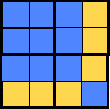
\includegraphics[width=0.19\textwidth]{signs}
                \end{center}
                \caption{The signs associated with a wavelet coefficient. Blue is positive and orange is negative; both magnitudes are one.  }
                \label{fig:signs}    
            \end{wrapfigure}

            We're given a randomly undersampled image and asked to approximate it's wavelet transform, a daunting task to the unexperienced. The unexperienced, myself, went through quite a process in figuring out how to do this. 

            First, some preface. We have $w = c x r$ where $w$ are the wavelet coefficients, $c$ the matrix that performs the wavelet transform on the columns, $r$ the rows and $x$ our 2D signal (an image in this case).

            I tried to make the approximation procedure similar to the 1D case. I tried deleting rows and columns from the two matrices from $c$ and $r$ as well as finer terms. I was hoping for a psuedo-inverse type situation, as in the 1D case.

            Before I tried this method, I was introduced to $\phi$ and $\psi$, the approximation and detail functions. I ignored these because they seemed to mathematical at the time, and too far in the clouds. I was guessing that it would be a much simpler operation.

            I'll introduce the basic equations now. I don't see a way around it.

            \begin{equation}
                \phi(n) = 
                \begin{cases}
                    1 & n=0,1 \\
                    0 & \mathrm{otherwise}
                \end{cases}
                \label{eq:phi}
            \end{equation}
            \begin{equation}
                \psi(n) = 
                \begin{cases}
                    1 & n=0 \\
                    -1 & n=1 \\
                    0 & \mathrm{otherwise}
                \end{cases}
                \label{eq:phi}
            \end{equation}

            These equations are just implement the Haar transform. You call $\phi$ and $\psi$ recursively, using the output from the previous example as input. But, they aren't scaled right. When you recursively call this function, you get a factor of $\sqrt{2}$. Then, this equation can also represent different powers and different shifts. We wind up calling...


            $$2^{-j/2}\phi(2^j x - k)$$
            
            There's a much better example at \cite{stollnitz1995wavelets}. It fully explains the powers and shifts: I just touched on it. For the powers, we can think of each function as having a different scale. Since it's at a different power, we need to have a different shift, since each one is uniquely localized. 

            But, that's just for the 1D case. Since we apply it to the rows and the columns, we have the 2D functions:

            $$ \phi\phi(x,y) = \phi(x) \phi(y) $$
            $$ \psi\phi(x,y) = \psi(x) \phi(y) $$
            $$ \phi\psi(x,y) = \phi(x) \psi(y) $$
            $$ \psi\psi(x,y) = \psi(x) \psi(y) $$

            These correspond to the four quadrants of an image: $A$, $V$, $D$, and $H$.

            %TODO: more stuff explaining

            The long and the short of it is that we have four samples (let's say):

            $$ w = h s $$

            $w$ are the approximations of the wavelet coefficients, $h$ some magic $N \times N$ matrix that represents a linear system, and $s$ our samples.

            \begin{equation}
                \begin{bmatrix}
                   w_A \\ w_H \\ w_V \\ w_D 
                \end{bmatrix}
                =
                \begin{bmatrix}
                    \phi\phi(x_{s_1},y_{s_1})& \phi\phi(x_{s_2},y_{s_2})&\phi\phi(x_{s_3},y_{s_3}) &\phi\phi(x_{s_4},y_{s_4})\\
                    \phi\psi(x_{s_1},y_{s_1})& \phi\psi(x_{s_2},y_{s_2})& \phi\psi(x_{s_3},y_{s_3})& \phi\psi(x_{s_4},y_{s_4})\\ 
                    \psi\phi(x_{s_1},y_{s_1})& \psi\phi(x_{s_2},y_{s_2})& \psi\phi(x_{s_3},y_{s_3})& \psi\phi(x_{s_4},y_{s_4})\\ 
                    \psi\psi(x_{s_1},y_{s_1})& \psi\psi(x_{s_2},y_{s_2})& \psi\psi(x_{s_3},y_{s_3})& \psi\phi(x_{s_4},y_{s_4})\\ 
                \end{bmatrix}
                \begin{bmatrix}
                   s_1 \\ s_2 \\ s_3 \\ s_4 
                \end{bmatrix}
                \label{eq:theeq}
            \end{equation}

            This is just saying that we know that the wavelet coefficients are just scaled properly and include those terms.

            The calling of $\phi$ and $\psi$ are simply putting \Cref{fig:signs} into a mathematical package.

        \subsection{The approximation algorithm}
        Yes, we know how to make the matrix: it's just full of $\phi$ and $\psi$ in the approbate places. $j$ is determined by the level of wavelet and $k,l$ are determined by where we are in the square (we have to look at how many shifts are possible and determine if $x,y$ is in that. 

        But the algorithm is a different story -- we have to write down \textbf{how} to tell what $j$ and $k$ are.

        \subsubsection{$j$ -- the power variable}
            This is easy. We know how far we are away from the top left corner and what power of wavelet we're going for.

        \subsubsection{$k$ -- the shift variable}
            This is slightly more complex. This involves both the power (how many shifts are possible?) and the $(x,y)$ position. But we know how far we are away from the upper left corner of the current quadrant (either in the $x$ or $y$ directions). We know that the number of shifts increases by one for each shift in position, making sense since the power is halfed each time.



        \subsection{Which indices are important?}
            Initially, I thought that the wavelet transform had to be recursive. That makes it really tricky for the indices -- you would have to make \texttt{dwt\_ind} functions, and keep doing it. 

            But after I talked to Ashkay, I learned that you can do the full wavelet transform on each row then each wavelet transform on each column. That makes this function trivial: it's just a matter of indexing. 

        \subsection{The reconstruction}
            In the wavelet domain, we have a tree that corresponds to the image. An example is in \Cref{fig:tree}. The upper levels of the tree represent the lower frequency terms. Since there's no need to closely sample a low frequency term, we only sample where there are high frequencies. 

            We know that if any of these ``branches'' are close enough to zero ($|x| < \lambda$) that all of it's child branches are close enough to 0 as well. Therefore, we only look at where the branches are not close enough to zero ($|x| > \lambda$). As we go further down the branch, we form a better approximation of the wavelet transform.
            
            \begin{figure}[h]
                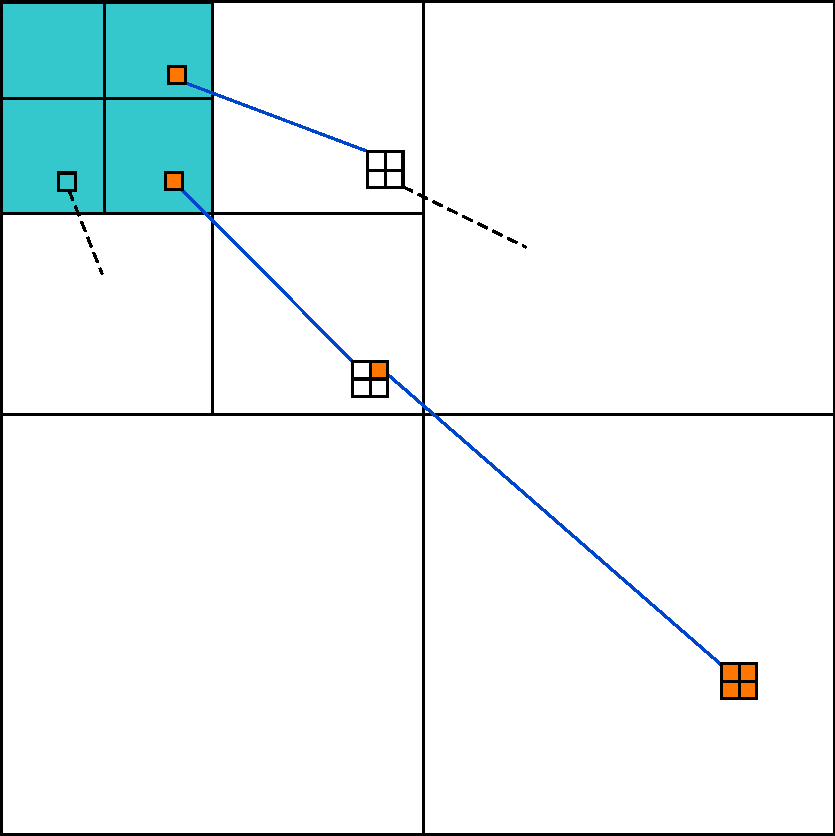
\includegraphics[angle=0]{better_diagram}
                \caption{A visualization of our tree. The blue square is our current node. Only two of it's components are non-zero, meaning that there's more detail at lower levels we need to look at closer. We then build a better and better approximation as we need too.}
                \label{fig:tree}
            \end{figure}
            
            Where we choose to look (or where we sample) is near the edges. The wavelet transform is zero for a constant: it has no high frequency terms.




            \bibliographystyle{plain}
            \bibliography{BibDesk}
            \printbibliography{}

\end{document}





































